%**************************
\chapter{Desarollo matemático}
\label{ch:Desarollo matemático}
%**************************

% TODO: conceptos
% conceptos han aparecido: extensión de cuerpo, característica, grupo, homomorfismo, clasura algebraica, orden, cardinal, núcleo, tª estructura gurpos abelianos..

% TODO: dudas
% tengo que saber los teoremas que he referenciado como el teorema de Bezout o el teorema de Rienman-Roch?
% bien la forma de citar?
% demo de estructura subgrupo de torsión

% TODO: completar introducción
En este capítulo haremos el estudio matemático de la teoría de curvas elípticas. En el apartado~\ref{sec:Teoría básica de curvas elípticas} se desarolla la teoría básica.
%, mientras que en el apartado~\ref{} se particulariza a curvas elítipcas sobre cuerpos finitos y por último en el apartado~\ref{} se ve...

% TODO: añadir ref si se utilizán más
Las referencias utilizadas para el desarollo matemático han sido sido~\cite{Washington:2008},~\cite{Hankerson:2003} y~\cite{Silverman:2009}.

\section{Teoría básica de curvas elípticas}
\label{sec:Teoría básica de curvas elípticas}

En este apartado se tratarán las ecuaciones de Weierstrass, las operaciones de adicción y duplicación, los puntos proyectivos, los endomorfismos de curvas elípticas y la estructura de los puntos de torsión.

Las principales referencias utilizadas en este capítulo han sido~\cite[cap. 2]{Washington:2008} y~\cite[cap. 3]{Hankerson:2003}.

\subsection{Definición de curva elíptica}
\label{sub:Definición de curva elíptica}

En esta apartado veremos la definición general de curva elíptica aunque posteriormente simplificaremos la ecuación que la define.

\begin{definicion}
\label{def:curva elíptica}
	Una \emph{curva elíptica} $E$ se define por una una ecuación de la forma
	\begin{equation}
	\label{eq:Weierstrass general}
		E : y^2 + a_1 x y + a_3 y = x^3 + a_2 x^2 + a_4 x + a_6
	\end{equation}

	donde $a_1, a_2, a_3, a_4, a_6 \in K$ y $\Delta \neq 0$, siendo $\Delta$ el \emph{discriminante} de $E$ y definiéndose como:

	\begin{align}
		\label{eq:discriminante}
		\begin{rcases}
		\Delta & = -d_2^2 d_8 - 8 d_4^3 - 27 d_6^2 + 9 d_2 d_4 d_6         \\
		d_2    & = a_1^2 + 4 a_ 2                                          \\
		d_4    & = 2 a_4 + 4 a_2                                           \\
		d_6    & = a_3^2 + 4 a_6                                           \\
		d_8    & = a_1^2 a_6 + 4 a_2 a_6 - a_1 a_3 a_4 + a_2 a_3^2 - a_4^2 \\
		\end{rcases}
	\end{align}

	Si $L$ es una extensión del cuerpo $K$, entonces el conjunto de puntos \emph{L-racionales} de $E$ es:
	$$
	E(L) = \{\infty\} \cup \{(x, y) \in L \times L: y^2 + a_1 x y + a_3 y = x^3 + a_2 x^2 + a_4 x + a_6 \}
	$$
\end{definicion}

\begin{nota}[comentarios de la definición~\ref{def:curva elíptica}]\leavevmode
	\begin{itemize}
		\item La ecuación~\eqref{eq:Weierstrass general} se conoce como la \emph{ecuación de Weierstrass}.
		\item Diremos que $E$ \emph{está definida sobre} $K$ y lo notaremos $E/K$. A $K$ lo llamaremos \emph{cuerpo base}.
		% TODO: rellenar ref
		\item La condición $\Delta \neq 0$ asegura que la curva elíptica no tenga puntos \emph{singulares}, esto es, puntos que anulen las derivadas parciales de la función polínomica
		$$
			f(x, y) = y^2 + a_1 x y + a_3 y - x^3 - a_2 x^2 - a_4 x - a_6
		$$
		asociada a la curva elíptica. Esto asegura que no haya puntos en los que la curva tenga dos o más rectas tangentes.
		\item El punto $\infty$ lo llararemos \emph{punto del infinito}. Es el único punto en la recta del infinito que satisface la forma proyectiva de la ecuación de Weierstrass (véase apartado~\ref{sub:Puntos proyectivos}).
	\end{itemize}
\end{nota}

\begin{ejemplo}[curvas elípticas sobre $\mathbb{R}$]
	Consideramos las curvas elípticas:
	\begin{align*}
		E_1: y^2 & = x^3 - x \\
		E_2: y^2 & = x^3 + x
	\end{align*}
	definidas sobre el cuerpo $\mathbb{R}$ de los números reales. Los puntos $E_1(\mathbb{R})$ y $E_2(\mathbb{R})$ se han representado en la Figura~\ref{fig:curvas elípticas reales}.

	\begin{figure}[h]
		\myfloatalign
		\subfloat[$E_1: y^2 = x^3 - x$]
		{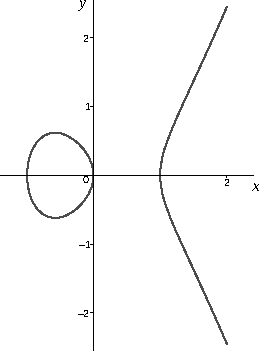
\includegraphics[width=.45\linewidth]{gfx/grafo_curva_eliptica_reales_1.pdf}} \quad
		\subfloat[$E_2: y^2 = x^3 + x$]
		{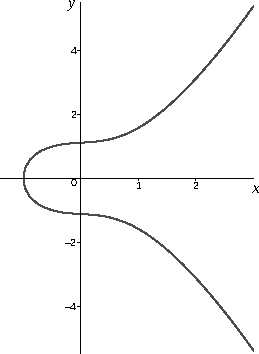
\includegraphics[width=.45\linewidth]{gfx/grafo_curva_eliptica_reales_2.pdf}}
		\caption{Curvas elípticas sobre $\mathbb{R}$}\label{fig:curvas elípticas reales}
	\end{figure}
\end{ejemplo}

\subsection{Ecuaciones de Weierstrass simplificadas}
\label{sub:Ecuaciones de Weierstrass simplificadas}

Nuestro objetivo es transformar la ecuación~\eqref{eq:Weierstrass general} por una ecuación más sencilla. En este apartado veremos varias transformaciones según la característica del cuerpo base.

\begin{definicion}
	Dos curvas elípticas $E_1$ y $E_2$ definidas sobre $K$ y dadas por las ecuaciones de Weierstrass:
	\begin{align*}
		E_1 &: y^2 + a_1 x y + a_3 y = x^3 + a_2 x^2 + a_4 x + a_6 \\
		E_2 &: y^2 + a_1' x y + a_3' y = x^3 + a_2' x^2 + a_4' x + a_6'
	\end{align*}
	se dicen que son \emph{isomorfas sobre K} si existen $u, r, s, t \in K,\ u \neq 0$, tal que el cambio de variables lineal
	\begin{equation}\label{eq:cambio de variables admisible}
	(x, y) \mapsto (u^2 x + r, u^3 y + u^2 s x + t)
	\end{equation}
	transforma la ecuación $E_1$ en la ecuación $E_2$. La transformación~\eqref{eq:cambio de variables admisible} se llama un cambio de variables admisible.

	El cambio de variables~\eqref{eq:cambio de variables admisible} es el único que deja <<fijo>> el punto del infinito y preserva la forma de la ecuación de Weierstrass. No vamos a entrar en más detalle, pero puede consultar~\cite[prop. III.3.1b]{Silverman:2009} para más informácion.
\end{definicion}

Una ecuación de Weierstrass
$$
E:  y^2 + a_1 x y + a_3 y = x^3 + a_2 x^2 + a_4 x + a_6
$$
puede simplificarse considerablemente aplicando cambios de variables admisibles. Veamos el caso en el que la característica del cuerpo base no es ni 2 ni 3.

\begin{lema}\label{lm: simplificación ecuación Weierstrass}
	Si $\car(K) \neq 2, 3$, entonces el cambio de variables admisible
	$$
	(x, y) \mapsto \left(\frac{x - 3 a_1^2 - 12 a_2}{36}, \frac{y - 3 a_1 x}{216} - \frac{a_1^3 + 4 a_1 a_2 - 12 a_3}{240}\right)
	$$
	transforma $E$ en la curva
	\begin{equation}\label{eq:ecuación Weierstrass}
		y^2 = x^3 + a x + b
	\end{equation}
	donde $a, b \in K$. El discriminante de esta curva es $\Delta = -16(4a^3 + 27b^2)$.
\end{lema}
\begin{proof}
Basta aplicar el cambio de variables y ver que efectivamente se obtiene la expresión~\eqref{eq:ecuación Weierstrass}. En su lugar, veamos el proceso por el cual se obtuvo dicha simplificación.

Dada la ecuación de Weierstrass~\eqref{eq:Weierstrass general}, sumamos en ambos lados por $(a_1 a_3 x)/2 + a_3^2/4 + (a_1^2 x^2)/4$ (podemos dividir por 2 ya que $\car(K) \neq 2$) para completar el cuadrado:
$$
\left(y + \frac{a_1 x}{2} + \frac{a_3}{2}\right)^2 = x^3 + \left(a_2 + \frac{a_1^2}{4}\right)x^2 + \left(a_4 + \frac{a_1 a_3}{2}\right)x + \left(a_6 + \frac{a_3^2}{4}\right)
$$
Haciendo $y_1 = y + (a_1 x)/2 + a_3/2$, obtenemos
$$
y_1^2 = x^3 + a_2' x^2 + a_4' x + a_6'
$$
para algunas constantes $a_2', a_4', a_6' \in K$. Finalmente, sustituyendo $x_1 = x + a_2'/3$ (podemos dividir por 3 ya que $\car(K) \neq 3$) resulta
$$
y_1^2 = x_1^3 + a x_1 + b
$$
para algunas constante $a, b \in K$. Para obtener el discriminante $\Delta$ basta sustiuir el valor de las constantes $a_4 = a,\ a_6 = b$ y $a_1 = a_3 = a_2 = 0$ en~\eqref{eq:discriminante}.
\end{proof}
\begin{nota}[comentarios del lema~\ref{lm: simplificación ecuación Weierstrass}] \leavevmode
	\begin{itemize}
		% TODO: rellenar ref
		\item Si el cuerpo base tiene característica 2, la ecuación anterior~\eqref{eq:ecuación Weierstrass} no es válida ya que tiene puntos singulares.
		\item Para cuerpos base con característica 3, la ecuación anterior~\eqref{eq:ecuación Weierstrass} si es válida, pero existan curvas que no tienen esta forma.
	\end{itemize}
\end{nota}

En la mayor parte del trabajo, desarollaremos la teoría de curvas elípticas utilizando la ecuación de Weierstrass simplificada~\eqref{eq:ecuación Weierstrass}. Sin embargo, como los cuerpos finitos de característica dos son de especial interés en computación, ocasionalmente señalaremos que modificaciones son necesarias para los cuerpos base de característica dos. Veamos la primera modificación.

\begin{lema}
	Si la característica de K es 2, hay dos casos que considerar. Si $a_1 \neq 0$, entonces el cambio de variables admisible
	$$
	(x, y) \mapsto \left(a_1^2 x + \frac{a_3}{a_1}, a_1^3 y + \frac{a_1^2 a_4 + a_3^2}{a_1^3} \right)
	$$
	transforma $E$ en la curva
	\begin{equation*}
		y^2 + xy = x^3 + a x^2 + b
	\end{equation*}
	% TODO: rellenar referencia
	donde $a, b \in K$. Tales curvas se llaman \emph{no supersingulares} (véase~\ref{}) y tienen discriminante $\Delta = b$. Si $a_1 = 0$, entonces el cambio de variables admisible
	$$
	(x, y) \mapsto (x + a_2, y)
	$$
	transforma $E$ en la curva
	\begin{equation*}
		y^2 + c y = x^3 + a x + b
	\end{equation*}
	% TODO: rellenar referencia
	donde $a, b, c \in K$. Tales curvas se llaman \emph{supersingulares} (véase~\ref{}) y tienen discriminante $\Delta = c^4$.
\end{lema}
\begin{proof}
	Basta sustituir el cambio de variables en la ecuación general de Weierstrass y operar.
\end{proof}


% Si la característica de $K$ es 3, entonces hay dos casos que considerar. Si $a_1^2 \neq -a_2$, entonces el cambio de variables admisible
% $$
% (x, y) \mapsto \left(x + \frac{d_4}{d_2}, y + a_1 x + a_1 \frac{d_4}{d_2} + a_3 \right)
% $$
% donde $d_2 = a_1^2 + a_2$ y $d_4 = a_4 - a_1 a_3$, transforma $E$ en la curva
% \begin{equation*}
% 	y^2 = x^3 + a x^2 + b
% \end{equation*}
% % TODO: rellenar referencia
% donde $a, b \in K$. Tales curvas se llaman \emph{no supersingulares} (véase~\ref{}) y tiene discriminante $\Delta = -a^3 b$. Si $a_1^2 = -a_2$, entonces el cambio de variables admisible
% $$
% (x, y) \mapsto (x, y + a_1 x + a_3)
% $$
% transforma $E$ en la curva
% \begin{equation*}
% 	y^2 = x^3 + a x^2 + b
% \end{equation*}
% % TODO: rellenar referencia
% donde $a, b \in K$. Tales curvas se llaman \emph{supersingulares} (véase~\ref{}) y tiene discriminante $\Delta = -a^3$.


\subsection{Ley de grupo}
\label{sub:Ley de grupo}

En este apartado veremos como dotar de estructura de grupo al conjunto de puntos una curva elíptica. Para ello definiremos una ley de composición o ley de grupo y le daremos sentido a la <<suma>> de puntos.

Sea $E$ una curva elíptica definida sobre un cuerpo $K$. El siguiente método geométrico permite dados dos puntos en $E(K)$ producir un tercero en $E(K)$. Este método será la base para definir la ley de grupo.

\begin{algoritmo}[Método de la cuerda y la tangente]
	Dados dos puntos $P$ y $Q$ , veamos como producir un tercer punto $R$. En primer lugar si $P$ y $Q$ son distintos, los pasos son:
	\begin{enumerate}
		\item Se dibuja una recta $L$ de $P$ a $Q$.
		\item Esta recta intersecta la curva elíptica en un tercer punto.
		\item Tomamos $R$ como la reflexión de este punto sobre el eje-$x$.
	\end{enumerate}
	Si los puntos $P$ y $Q$ son iguales, los pasos son:
	\begin{enumerate}
		\item Se dibuja la línea tangente $L$ a la curva elíptica en $P$.
		\item Esta línea intersecta la curva elíptica en un segundo punto.
		\item Tomamos $R$ como la reflexión de este punto sobre el eje-$x$.
	\end{enumerate}
	Esto método se puede apreciar en la figura~\ref{fig:Método de la cuerda y la tangente}.
\end{algoritmo}

\begin{figure}[h]
  \myfloatalign
  {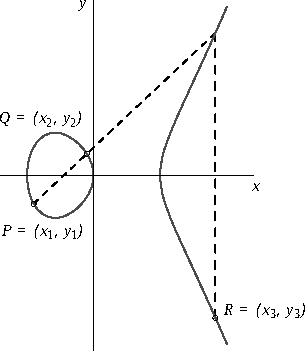
\includegraphics[width=.45\linewidth]{gfx/ejemplo_adiccion.pdf}}
  \quad
  {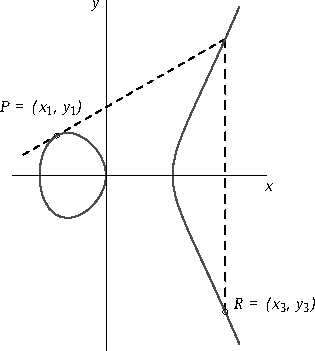
\includegraphics[width=.45\linewidth]{gfx/ejemplo_duplicacion.pdf}}
  \caption{Método de la cuerda y la tangente}\label{fig:Método de la cuerda y la tangente}
\end{figure}

\begin{nota}[comentarios del algoritmo~\ref{al:multiplicación por duplicación}]
El hecho de que $L \cap E$, contando multiplicidades, consiste en exactamente tres puntos (no necesariamente distintos) es un caso especial del teorema de Bézout~\cite[sec. I.7.8]{Hartshorne:1977}. Sin embargo, como a continuación vamos a dar fórmulas explícitas, haremos la demostración utilizando dichas fórmulas y no será necesario utilizar un teorema tan general.
\end{nota}

Inspirándonos en el método de la cuerda y la tangente, definimos la siguiente ley de composición para el grupo de puntos de una curva elíptica.

\begin{definicion}[ley de grupo]
\label{def:ley de grupo}
Sea $E$ una curva elíptica definida por la ecuación $y^2 = x^3 + a x + b$ sobre un cuerpo $K$ de característica distinta de 2 y 3. Definimos la operación binaria $+: E(K) \times E(K) \to E(K)$ como sigue:
\begin{enumerate}[label=\alph*)]
	\item $P + \infty = \infty + P = P,$ para todo $P \in E(K)$
	\item Si $P = (x, y) \in E(K)$, entonces $(x, y) + (x, -y) = \infty$. El punto $(x, -y)$ se denotará por $-P$ y se llamará el \emph{opuesto} de P. Además, $- \infty = \infty$.
	\item Sea $P = (x_1, y_1) \in E(K)$ y $Q = (x_2, y_2) \in E(K)$, donde $P \neq \pm Q$. Entonces $P + Q = (x_3, y_3)$, donde
	$$
	x_3 = \left(\frac{y_2 - y_1}{x_2 - x_1}\right)^2 - x_1 - x_2, \quad
	y_3 = \left(\frac{y_2 - y_1}{x_2 - x_1}\right) (x_1 - x_3) - y_1
	$$
	\item Sea $P = (x_1, y_1) \in E(K)$, donde $P \neq  -P$. Entonces $2 P = (x_3, y_3)$ donde:
	$$
	x_3 = \left(\frac{3 x_1^2 + a}{2 y_1}\right)^2 - 2 x_1, \quad
	y_3 = \left(\frac{3 x_1^2 + a}{2 y_1}\right) (x_1 - x_3) - y_1
	$$
\end{enumerate}
\end{definicion}
\begin{proof}
Tenemos que comprobar que $+$ es una operación binaria válida, esto es, que a cada par de elementos de $E(K) \times E(K)$ le corresponde un único elemento de $E(K)$. Como la casuística anterior es total y exclusiva, basta ver que $+$ es una operación cerrada. Los casos $a)$ y $b)$ son triviales. Veamos los otros dos casos con detalle.

\paragraph{Caso $c)$}
Supongamos $P = (x_1, y_1),\ Q = (x_2, y_2),\ P, Q \in E(K)$ con $P \neq \pm Q$. Consideramos la recta que los contiene:
$$
	L: y = m(x - x_1) + y_1,\ \text{donde}\ m = \frac{y_2 - y_1}{x_2 - x_1}
$$
Nótese que $x_2 \neq x_1$ ya que $P \neq \pm Q$. Para hallar la intersección de L con E sustituimos $y$:
$$
	(m(x - x_1) + y_1)^2 = x^3 + a x + b
$$
Podemos reescribir esto de la forma
\begin{equation}
\label{eq:cúbica}
	0 = x^3 - m^2 x^2 + b' x + c'
\end{equation}
para algunas constantes $b', c' \in K$. Así, las raíces de esta cúbica es justamente $L \cup E$.

Sabemos que las raíces de un polinomio están relacionadas con sus coeficientes. De hecho, para un polinomio cúbico mónico $x^3 + c_2 x^2 + c_1 x + c_0$ con raíces $r, s, t$ se tiene:
% -r s t  +  r s x  +  r t x  -  r x^2  +  s t x  -  s x^2  -  t x^2+x^3
\begin{align*}
	x^3 + &c_2 x^2 + c_1 x + c_0 = (x-r)(x-s)(x-t) \\
	&= x^3 - (r + s + t)x^2 + (r s + r t + s t)x - r s t
\end{align*}

En particular, $r + s + t = -c_2$. Como $P$ y $Q$ están en la intersección, $x_1$ y $x_2$ son dos raíces de~\eqref{eq:cúbica}, luego la tercera raíz $\alpha$ es $m^2 - x_1 - x_2$. Sustituyendo $\alpha$ en $L$ resulta $\beta = m(x_3 - x_1) + y_1$, luego $(\alpha, \beta) \in E(K)$. Entonces  $(\alpha, -\beta) = (x_3, y_3) \in E(K)$.

\paragraph{Caso $d)$}
Sea $P = (x_1, y_1)$, donde $P \neq -P$. Consideramos la recta tangente a $E$ en $P$
$$
	L: y = m(x - x_1) + y_1,\ \text{donde}\ m = \frac{3 x_1^2 + a}{2 y_1}
$$
Nótese que $y_1 \neq 0$ ya que si no estaríamos en el caso $b)$. Hallamos la intersección con E de forma análoga al caso $c)$ y obtenemos la cúbica:
$$
	0 = x^3 - m^2 x^2 + b' x + c'
$$
para algunas constantes $b', c' \in K$. Análogamente al caso $c)$, como $x_1$ es una raíz doble de la cúbica (derívese y evalúe en $x_1$) tenemos que la tercera raíz $\alpha$ es $m^2 - 2 x_1$. Sustituyendo $\alpha$ en $L$ resulta $\beta = m(x_3 - x_1) + y_1$, luego $(\alpha, \beta) \in E(K)$. Entonces  $(\alpha, -\beta) = (x_3, y_3) \in E(K)$.
\end{proof}

\begin{nota}[comentarios de la definición~\ref{def:ley de grupo}]
	Para cuerpos base con característica 2 o 3, las fórmulas cambian. Por ejemplo, si $E$ es una curva elíptica definida sobre un cuerpo $K$ por la ecuación general de Weierstrass~\eqref{eq:Weierstrass general}, el opuesto de un punto $P = (x, y) \in E(K)$ viene dado por
	$$
		- P = (x, -a_1 x - a_3 - y)
	$$
	% TODO: rellenar ref
	En el apartado~\ref{} veremos la ley de composición para una curva elíptica sobre un cuerpo finito de característica 2.
\end{nota}

Con la operación binaria~\ref{def:ley de grupo}, el conjunto de puntos de una curva elíptiptica es un grupo abeliano.

\begin{teorema}\label{th:grupo abeliano}
	La suma~\ref{def:ley de grupo} de puntos en una curva elíptica $E$ sobre un cuerpo $K$ de característica distinta de 2 y 3 satisface la siguientes propiedades:
	\begin{itemize}
		\item \emph{Conmutatividad.} $P_1 + P_2 = P_2 + P_1,\ \forall P_1, P_2 \in E(K)$.
		\item \emph{Existencia de elemento neutro.} $P + \infty = P,\ \forall P \in E(K)$.
		\item \emph{Existencia de elemento opuesto.} $P + (-P) = \infty,\ \forall P \in E(K)$.
		\item \emph{Asociatividad.} $(P_1 + P_2) + P_3 = P_1 + (P_2 + P_3),\ \forall P_1, P_2, P_3 \in E(K)$.
	\end{itemize}
	En otras palabras, $(E(K), +, \infty)$ es un grupo abeliano.
\end{teorema}
\begin{proof}
La conmutatividad es trivial en los casos $a)$, $b)$ y $d)$. Para el caso $c)$ también es fácil ya que la recta que une $P_1$ y $P_2$ es la misma que la recta que une $P_2$ y $P_1$. La existencia de elemento neutro e inverso también es directo de la definición~\ref{def:ley de grupo}.

La asociatividad puede probarse utilizando las fórmulas caso por caso, pero supone un esfuerzo demasiado laborioso. En su lugar, puede abordarse de forma más sofisticada bien estudiando las líneas y sus intersecciones con la curva elíptica en el plano proyectivo~\cite[sec. 2.4]{Washington:2008} o bien usando teoremas más generales como el de Riemann-Roch~\cite[teo. III.3.4.e]{Silverman:2009}.
\end{proof}

\begin{nota}[comentarios del teorema~\ref{th:grupo abeliano}]
	Puede encontrar una versión más general del teorema anterior para cuerpos bases de cualquiera característica en ~\cite{Silverman:2009}.
\end{nota}

% TODO: poner en el apartado cuerpos finitos
% TODO: poner tambien las supersingulares
% \begin{definicion}[ley de grupo 2]
% \label{def:ley de grupo 2}
% Sea $E$ una curva elíptica definida por la ecuación $y^2 + x y = x^3 + a x^2 + b$ sobre el cuerpo finito $\Fm$. Definimos la operación binaria $+: E(\Fm) \times E(\Fm) \to E(\Fm)$ como sigue:
% \begin{enumerate}[label=\alph*)]
% 	\item $P + \infty = \infty + P = P,$ para todo $P \in E(\Fm)$
% 	\item Si $P = (x, y) \in E(\Fm)$, entonces $(x, y) + (x, x + y) = \infty$. El punto $(x, x + y)$ se denotará por $-P$ y se llamará el \emph{opuesto} de P. Además, $- \infty = \infty$.
% 	\item Sea $P = (x_1, y_1) \in E(\Fm)$ y $Q = (x_2, y_2) \in E(\Fm)$, donde $P \neq \pm Q$. Entonces $P + Q = (x_3, y_3)$, donde
% 	$$
% 	x_3 = \lambda^2 \lambda + x_1 + x_2 + a, \quad
% 	y_3 = \lambda (x_1 + x_3) + x_3 + y_1
% 	$$
% 	con $\lambda = (y_1 + y_2)/(x_1 + x_2)$.
% 	\item Sea $P = (x_1, y_1) \in E(\Fm)$, donde $P \neq -P$. Entonces $2 P = (x_3, y_3)$ donde:
% 	$$
% 	x_3 = \lambda^2 \lambda + a = x_1^2 + b/x_1^2, \quad
% 	y_3 = x_1^2 + \lambda x_3 + x_3
% 	$$
% 	con $\lambda = x_1 + y_1/x_1$.
% \end{enumerate}
% \end{definicion}
%
% \begin{teorema}
% 	La suma~\ref{def:ley de grupo 2} de puntos en una curva elíptica $E$ sobre el cuerpo $\F2m$ satisface la siguientes propiedades:
% 	\begin{itemize}
% 		\item \emph{Conmutatividad.} $P_1 + P_2 = P_2 + P_1,\ \forall P_1, P_2 \in E(F2m)$.
% 		\item \emph{Existencia de elemento neutro.} $P + \infty = P,\ \forall P \in E(F2m)$.
% 		\item \emph{Existencia de elemento opuesto.} $P + (-P) = \infty,\ \forall P \in E(F2m)$.
% 		\item \emph{Asociatividad.} $(P_1 + P_2) + P_3 = P_1 + (P_2 + P_3),\ \forall P_1, P_2, P_3 \in E(F2m)$.
% 	\end{itemize}
% 	En otras palabras, $(E(F2m), +, \infty)$ es un grupo abeliano.
% \end{teorema}


\subsection{Multiplicación escalar}
\label{sub:Multiplicación escalar}

En este apartado veremos un método eficiente para calcular la duplicación reiterada de un punto.

Sea $P$ es un punto de una curva elíptica y $k$ un entero positivo. Denotaremos $k P$ a la suma $P + \ldots + P$ de $k$-sumandos. El siguiente algoritmo calcula $k P$ más rápido que el método directo (sumar $P$ consigo mismo repetidamente).

\begin{algoritmo}[multiplicación por duplicación]\label{al:multiplicación por duplicación}
	Sea $k$ un entero positivo y sea $P$ un punto de una curva elíptica. El siguiente algoritmo calcula $kP$.
	\begin{enumerate}
		\item Se empieza con $a = k$, $B = \infty$ y $C = P$.
		\item Si $a$ es par, se toma $a = a/2$, $B = B$ y $C = 2 C$.
		\item Si $a$ es impar, se toma $a = a -1$, $B = B + C$ y $C = C$.
		\item Si $a \neq 0$, se va al paso 2.
		\item Se devuelve $B$.
	\end{enumerate}
	La salida $B$ es $kP$.
\end{algoritmo}

\begin{nota}[comentarios del algoritmo~\ref{al:multiplicación por duplicación}]\leavevmode
	\begin{itemize}
		\item El único problema de este método es que el tamaño de las coordenadas incrementa muy rápidamente.
		\item Si trabajos sobre un cuerpo finito, podemos evitar este incoveniente reduciendo módulo $p$ en cada operación.
	\end{itemize}
\end{nota}

\subsection{Puntos proyectivos}
\label{sub:Puntos proyectivos}

En este apartado introduciremos los puntos proyectivos y veremos de donde procede el punto del infinito de una curva elíptica. Como en la mayor parte del trabajo no vamos a trabajar con puntos proyectivos, veremos este apartado de manera más informal.

Sea $K$ un cuerpo. El \emph{espacio proyectivo} dos dimensional sobre $K$, $\P^2(K)$, esta dado por clases de equivalencia de ternas $(x, y, z)$ con $x, y, z \in K$ y al menos algún $x, y, z$ no nulo. Dos ternas $(x_1, y_1, z_1)$ y $(x_2, y_2, z_2)$ se dicen que son \emph{equivalentes} si existe un elemento no nulo $\lambda \in K$ tal que
$$
	(x_1, y_1, z_1) = (\lambda x_2, \lambda y_2, \lambda z_3)
$$
y en tal caso escribiremos $(x_1, y_1, z_1) \sim (x_2, y_2, z_2)$. La clase de equivalencia de una terna solo depende de los ratios entre $x, y, z$. Por ello, la clase de equivalencia de $(x, y, z)$ la denotaremos por $(x : y : z)$ y diremos que es un \emph{punto proyectivo}.

Si $(x : y : z)$ es un punto proyectivo con $z \neq 0$, entonces $(x : y : z) = (x/z : y/z : 1)$ y de hecho $(x/z, y/z, 1)$ es el único representante de esta clase de equivalencia con $z = 1$. Tenemos así una correspondencia $1-1$ entre el conjunto de puntos proyectivos
$$
	\P^2(K)^* = \left\{(x : y : z) : x, y, z \in K,\ z \neq 0 \right\}
$$
y el \emph{plano afín}
$$
	\A(K) = \left\{(x, y) : x, y \in K \right\}.
$$

Si $z = 0$, el conjunto de puntos proyectivos de la forma $(x : y : 0)$ se llaman \emph{recta del infinito} ya que sus puntos no se corresponden con ningúno del plano afín.

La \emph{forma proyectiva} de una ecuación de Weierstrass de una curva elíptica $E$ definida sobre $K$ se obtiene remplazando $x$ por $x/z$, $y$ por $y/z$ y quitando denominadores. Si alguna terna $(x, y, z)$ no nula satisface la ecuación proyectiva entonces también las satisfacen las ternas $(x', y', z') \in (x : y : z)$. Podemos decir entonces que un punto proyectivo $(x : y : z)$ está en $E$. Tenemos así una correspondencia 1-1 entre los puntos del plano afín que están en $E$ y los puntos proyectivos de $P^2(K)^*$ que están en $E$.

Si hacemos $z = 0$ en la forma proyectiva de la ecuación, obtenemos $0 = x^3$ y como alguna componente tiene que ser no nula, tenemos $y \neq 0$. Así, el único punto de la recta del infinito que está en $E$ es el punto $(0 : y : 0) = (0 : 1 : 0)$. Este pusto se corresponde con el punto $\infty$ de la definición~\ref{def:curva elíptica}.

Hay situaciones en la que usar coordenadas proyectivas puede ser ventajoso (véase~\cite[sec 2.6]{Washington:2008}). Sin embargo, nosotros utilizaremos las coordenadas del plano afín y trataremos el punto del infinito como caso especial cuando sea necesario.

% TODO: decidir si poner algo
% \subsection{El j-invariante}
% \label{sub:El j-invariante}

\subsection{Endomorfismos}
\label{sub:Endomorfismos}

% TODO: añadir ref
El principal objetivo de este apartado es probar la proposición~\ref{pp:cardinal del núcleo} que será utilizada en la demostración del teorema de Hasse~\ref{}. Para ello, es necesario utilizar algunos resultados técnicos, los cuales solo los enunciaremos (puede encontrar su demostración en ~\cite[sec. 2.9]{Washington:2008} ).

% En este apartado, $E$ denotará una curva elíptica definida sobre un cuerpo $K$ de característica distinta de 2 y 3 y definida por la ecuación de Weierstrass simplificada $y^2 = x^3 + a x + b$. Para curvas elípticas sobre cuerpos de características 2 o 3 o definidos por la ecuación general de Weierstrass las ideas son las mismas, por lo

\begin{definicion}
	Sea $E$ una curva elíptica definida sobre un cuerpo $K$ y sea $\Kca$ su clasura algebraica. Un \emph{endomorfismo} de $E$ es un homomorfismo $\alpha: \EKca \to \EKca$ dado por funciones racionales (cocientes de polinomios). Dicho de otro modo, $\alpha$ preserva la suma y el elemento neutro de $\EKca$.

	El endomorfismo trivial que lleva cada punto a $\infty$ lo denotaremos por 0.
\end{definicion}

Supondremos que $\alpha$ es no trivial a partir de ahora. El siguiente resultado técnico nos facilitará el manejo de endomorfismos de una curva elíptica.

\begin{lema}\label{lm:endomorfismo con funciones racionales}
	Si $\alpha$ es un endomorfismo de una curva elíptica definida por la ecuación de Weierstrass simplificada~\eqref{eq:ecuación Weierstrass}, entonces $\alpha$ se puede escribir como
	$$
	\alpha(x, y) = (r_1(x), r_2(x) y)
	$$
	donde
	\begin{itemize}
		\item $r_1(x) = p(x) / q(x)$, con $p(x), q(x)$ polinomios sin factores comunes.
		\item Si $q(x) = 0$ para algún punto $(x, y)$, entonces definimos $\alpha(x, y) = \infty$.
		\item Si $q(x) \neq 0$, entonces $r_2(x)$ está definida.
	\end{itemize}
\end{lema}

\begin{definicion}
	El \emph{grado} de un endomorfismo $\alpha$ es
	$$
		\dega= \max \{ \deg p(x) , \deg q(x) \}
	$$
	si $\alpha$ es no trivial. Si $\alpha = 0$, definimos $\deg(0) = 0$.
\end{definicion}

\begin{definicion}
	Un endomorfismo $\alpha$ no trivial es \emph{separable} si la derivada $r_1(x)'$ no es idénticamente cero.

	% En cuerpos con característica cero, un polinomio no constante siempre tendrá derivada no nula. En cuerpos de característica $p > 0$, los polinomios con derivada nula son exactamente aquellos de la forma $g(x^p)$.
\end{definicion}

% TODO: rellenar ref
El siguiente resultado será crucial en la demostración del teorema de Hasse~\ref{}. Denotaremos por  $\left\vert{C}\right\vert$ al número de elementos de un conjunto $C$.

\begin{proposicion}\label{pp:cardinal del núcleo}
	Sea $\alpha \neq 0$ un endomorfismo separable de una curva elíptica $E$. Entonces
	$$
		\dega = \left\vert{\ker(\alpha)}\right\vert
	$$
	donde $\ker(\alpha)$ es el núcleo del homomorfismo $\alpha : \EKca \to \EKca$. Si $\alpha \neq 0$ no es separable, entonces
	$$
		\dega > \left\vert{\ker(\alpha)}\right\vert
	$$
\end{proposicion}
\begin{proof}
	Por el lema~\ref{lm:endomorfismo con funciones racionales}, $\alpha(x, y) = (r_1(x), r_2(x) y)$ con $r_1(x) = p(x) / q(x)$. Supongamo que $\alpha$ es separable. Entonces $r_1' \neq 0$, por lo que $p' q - p q'$ no es el polinomio cero.

	Sea $S$ el conjunto de $x \in \Kca$ tal que $(p q' - p' q)(x) q(x) = 0$. Sea $(u, v) \in \EKca$ tal que
	\begin{enumerate}
		\item $u \neq 0,\ v \neq 0,\ (u, v) \neq \infty$,
		\item $\deg (p(x) - u q(x) ) = \max \{ \deg(p), \deg(q) \} = \dega$,
		\item $u \not\in r_1(S)$ y
		\item $(u, v) \in \alpha(\EKca)$.
	\end{enumerate}
	Como $p' q - p q'$ no es el polinomio nulo, $S$ es un conjunto finito, por lo que su imagen bajo $\alpha$ es finita. Por otro lado $\alpha(\EKca)$ es un conjunto infinito. Así, tal $(u, v)$ existe.

	Veamos que existen exactamente $\dega$ puntos $(x_1, y_1) \in \EKca$ tal que $\alpha(x_1, y_1) = (u, v)$. Para tales puntos, se tiene
	$$
	\frac{p(x_1)}{q(x_1)} = u, \quad y_1 r_2(x_1) = v
	$$
	Como $(u, v) \neq \infty$, $q(x_1) \neq 0$ luego $r_2(x_1)$ está definido. Como $v \neq 0$ y $y_1 r_2(x_1) = v$, se tendrá $y_1 = v/r_2(x_1)$, esto es, $x_1$ determina $y_1$, por lo que solo tenemos que contar valores de $x_1$.

	Por la propiedad (2), $p(x) - u q(x)$ tiene $\dega$ raíces, contando multiplicidades. Tenemos que ver que $p - u q$ no tiene raíces múltiples. Supongamos que $x_0$ es una raíz múltiple. Entonces
	$$
		p(x_0) - u q(x_0) = 0, \quad p'(x_0) - u q'(x_0) = 0
	$$
	Multiplicando las ecuaciones $p = u q$ y $u q' = p'$ resulta
	$$
		u p(x_0) q'(x_0) = u p'(x_0) q(x_0)
	$$
	Como $u \neq 0$, esto implica que $x_0$ es una raíz de $p q' - p' q$, por lo que $x_0 \in S$. Así $u = r_1(x_0) \in r_1(S)$, contrario u la propiedad (3). Concluimos que $p - u q$ no tiene raíces múltiples y por ello tiene $\dega$ raíces distintas.

	Como hay exactamente $\dega$ puntos $(x_1, y_1)$ con $\alpha(x_1, y_1) = (u, v)$, el núcleo de $\alpha$ tiene $\dega$ elementos.

	Nótese que como $\alpha$ es un homomorfismo, para cada $(u, v) \in \alpha(\EKca)$ hay exactamente $\dega$ puntos $(x_1, y_1)$ con $\alpha(x_1, y_1) = (u, v)$. Las hipótesis sobre $(u, v)$ se hicieron para obtener el resultado para al menos un punto, lo cual es suficiente.

	Si $\alpha$ no es separable, entonces los pasos de la demostración siguen siendo válidos, excepto que $p' - u q'$ es siempre el polinomio cero en este caso, por lo que $p(x) - u q(x) = 0$ tiene siempre raíces múltiplces y por ello tiene menos de $\dega$ soluciones.
\end{proof}

% TODO: ref
Veamos un par de resultados que serán útiles para describir la estructura de los puntos de torsión del apartado ~\ref{}.

\begin{proposicion}\label{pp:sobreyectividad endomorfismos}
	Sea $E$ una curva elíptica definida sobre el cuerpo $K$. Sea $\alpha \neq 0$ un endomorfismo de $E$. Entonces $\alpha$ es sobreyectiva.
\end{proposicion}
\begin{proof}
Sea $(u, v) \in \EKca$. Como $\alpha(\infty) = \infty$, supongamos que $(u, v) \neq \infty$. Por el lema~\ref{lm:endomorfismo con funciones racionales}, $\alpha$ será de la forma $\alpha(x, y) = (r_1(x), r_2(x) y)$ con $r_1(x) = p(x) / q(x)$. Consideramos el polinomio $p(x) - u q(x)$. Distinguimos dos casos.

Supongamos que $p(x) - u q(x)$ no es un polinomio constante. Entonces tendrá una raíz $x_0$. Como $p$ y $q$ no tiene raíces en común, $q(x_0) \neq 0$. Sea $y_0 \in \Kca$ una raíz cuadrada de $x_0^3 + u x_0 + v$. Como $q(x_0) \neq 0$, $r_2(x)$ está definido y por lo tanto $\alpha(x_0, y_0)$ también y valdrá $(u, v')$ para algún $v'$. Como $v'^2 = u^3 + a u + b = v^2$, tenemos $v' = \pm v$. Si $v' = v$, hemos terminado. Si $v' = -v$, entonces $\alpha(x_0, -y_0) = (u, -v') = (u, v)$.

Supongamos que $p - uq$ es un polinomio constante. Como $\EKca$ no es finito y el núcleo de $\alpha$ sí es finito, solo un número finito de puntos de $\EKca$ puede tener como imagen un punto con una componente $x$ dada. Así, bien $p(x)$ o $q(x)$ no es constante. Si $p$ y $q$ son dos polinomios no constantes, entonces hay como mucho una constante $u$ tal que $p - uq$ es constante (si $u'$ fuera otra constante que lo verificara, se tendría $(u' - u)q = (p - u q) - (p - u' q)$ es constante y $(u - u') p = u' (p - u q) - u (p - u' q)$ es constante, lo que implicaría que $p$ y $q$ son constantes). Así, hay al menos dos puntos, $(u, v)$ y $(u, -v)$ para algún $v$, que no están en la imagen de $\alpha$. Sea $(u_1, v_1)$ otro punto. Entonces $\alpha(P_1) = (u_1, v_1)$ para algún $P_1$. Podemos elegir $(u_1, v_1)$ tal que $(u_1, v_1) + (u, v) \neq (u, \pm v)$, por lo que existe $P_2$ con $\alpha(P_2) = (u_1, v_1) + (u, v)$. Entonces $\alpha(P_2 - P_1) = (u, v)$ y $\alpha(P_1 - P_2) = (u, -v)$.

\end{proof}

% TODO: ver si especificar el resultado para cuerpos base de car != 2
\begin{proposicion}\label{pp:endomorfismo multiplicación}
	Sea $E$ una curva elíptica definida sobre un cuerpo $K$ y sea $n$ un entero no cero. Consideramos el endomorfismo \emph{multiplicación} por $n$  dado por
	$$
		n(P) = n P,\ \forall P \in \EKca
	$$
	Supongamos que está dado por funciones racionales $R_n$ y $S_n$, esto es,
	$$
		n(x, y) = (R_n(x), y S_n(x))
	$$
	para todo $(x, y) \in \EKca$. Entonces
	$$
		\frac{R_n'(x)}{S_n(x)} = n.
	$$
	Por tanto, la multiplicación por $n$ es separable si y sólo si $n$ no es un múltiplo de la característica del cuerpo base.
\end{proposicion}

Para demostrar esta proposición, necesitamos un resultado técnico. La demostración de este lema se puede encontrar en~\cite[sec 2.9]{Washington:2008}.

\begin{lema}
	Sean $\alpha_1,\ \alpha_2,\ \alpha_3$ endomorfismos no triviales de una curva elíptica $E$ con $\alpha_1 + \alpha_2 = \alpha_3$. Supongamos que cada endomorfismo está dado de la siguiente forma
	$$
		\alpha_j(x, y) = (R_{\alpha_j}(x), y S_{\alpha_j}(x))
	$$
	y que existen constantes $c_{\alpha_1}, c_{\alpha_2}$ tal que
	$$
		\frac{R_{\alpha_1}'(x)}{S_{\alpha_1}(x)} = c_{\alpha_1}, \quad  \frac{R_{\alpha_2}'(x)}{S_{\alpha_2}(x)} = c_{\alpha_2}.
	$$
	Entonces
	$$
		\frac{R_{\alpha_3}'(x)}{S_{\alpha_3}(x)} = c_{\alpha_3} + c_{\alpha_3}
	$$
\end{lema}

\begin{proof}[Demostración de la proposición~\ref{pp:endomorfismo multiplicación}]
Dado un endomorfismo cualquiera $\alpha$, se tiene
$$
	\alpha(x, -y) = \alpha(-(x, y)) = - \alpha(x, y).
$$
En particular, $R_{-n} = R_n$ y $S_{-n} = -S_n$. Luego $R_n' / S_n = - R_n' / S_n$ y basta probar el resultado para $n$ positivos.

Para $n = 1$, la primera parte de la proposición es cierta. Aplicando el lema anterior, si es cierta para $n$, también es cierta para $n +1$ (la suma de $n$ y 1). Así,
$$
	\frac{R_n'(x)}{S_n(x)} = n.
$$
Por otro lado, $R_n'(x) \neq 0$ si y solo si $R_n'(x) / S_n(x) \neq 0$, que es equivalente a que la característica de $K$ no divida a $n$. Por la definición de separabilidad, esto prueba la segunda parte.
\end{proof}

% TODO: ver si meter el resto de resultados de endomorfismo
% TODO: ver donde meter frobenius
% Un importante ejemplo de endomorfismo es el \emph{endomorfismo de Frobenius}. Sea $E$ una curva elíptica definida sobre un cuerpo finito $\Fq$. El endomorfismo de Frobenius $\phi_q(x, y)$ está dado por
% $$
% 	\phi_q(x, y) = (x^q, y^q)
% $$

\subsection{Puntos de torsión}
\label{sub:Puntos de torsión}

% TODO: rellenar ref
En este apartado introduciremos los puntos de torsión y su estructura que jugarán un papel importante en las curvas elípticas sobre cuerpos finitos. También veremos el emparejamiento Weil el cual utilizaremos en la demostración del teorema de Hasse~\ref{}.

\begin{definicion}
	Dada una curva elíptica $E$, un elemento del grupo $\EKca$ cuyo orden es finito se llamará \emph{punto de torsión}.
\end{definicion}

\begin{definicion}
	Llamaremos \emph{subgrupo de n-torsión} al subgrupo de puntos $\Kca$-racionales
	$$
		E[n] = \{ P \in \EKca \ | \  n P = \infty \}.
	$$
	Estos conjuntos son subgrupos ya que son los núcleos del endomorfismo multiplicación por $n$ (definido en el apartado~\ref{sub:Endomorfismos}).
\end{definicion}

% TODO: ver que hacer
% Para describir la estructura de los subgrupos de torsión, necesitamos estudiar el endomorfismo multiplicación por un entero $n$. Los siguientes resultados nos darán las herramientas para probar el teorema~\ref{}. No es el objetivo de este trabajo la demostración de~\ref{} y~\ref{}, resultados técnicos y laboriosos, pero si está interesado puede encontrar sus demostraciones en~\cite[sec. 3.2]{Washington:2008}.
%
% \begin{proposicion}
% 	Sea $P = (x, y)$ un punto de la curva elíptica $y^2 = x^3 + a x + b$ sobre un cuerpo de característica distinta de 2 y sea $n$ un entero positivo. Entonces
% 	$$
% 		n P = (r(x), y s(x))
% 	%	n P = \left( \frac{\phi_n(x)}{\psi_n^2(x)} , \frac{\omega_n(x, y)}{\psi_n(x, y)^3} \right)
% 	$$
% \end{proposicion}

La \emph{suma directa} de dos grupos $G_1$ y $G_2$ la denotaremos $G_1 \oplus G_2$.

\begin{teorema}\label{th:estructura subgrupos torsión}
	Sea $E$ una curva elíptica sobre un cuerpo $K$ y sea $n$ un entero positivo. Si la característica de $K$ no divide a $n$, o es cero, entonces
	$$
		E[n] \simeq \mathbb{Z}_n \oplus \mathbb{Z}_n.
	$$
	Si la característica de $K$ es $p > 0$ y $p | n$, entonces
	$$
		E[n] \simeq \mathbb{Z}_{n'} \oplus \mathbb{Z}_{n'} \ \textrm{o} \ \simeq \mathbb{Z}_{n} \oplus \mathbb{Z}_{n'}
	$$
	donde $n = p^r n'$ con $p \nmid n'$.
\end{teorema}

% TODO: ver si no hay problema
Para demostrar este teorema vamos a usar un resultado cuya demostración técnica, extensa y laboriosa omitiremos. Puede consultar su demostración en~\cite[sec. 3.2]{Washington:2008}.

\begin{proposicion}\label{pp:grado endomorfismo multiplicación}
	Sea $E$ una curva elíptica. El endomorfismo multiplicación por $n$ de $E$ tiene grado $n^2$.
\end{proposicion}

\begin{proof}[Demostración del teorema~\ref{th:estructura subgrupos torsión}]
% TODO: puedo usar el endomorfismo multiplicación?
Supongamos primero que $n$ no es múltiplo de la característica $p$ del cuerpo. Por la proposicion~\ref{pp:endomorfismo multiplicación}, como $n$ no es múltiplo de la característica $p$, el endomorfismo multiplicación por $n$ es separable. Por la proposición~\ref{pp:cardinal del núcleo} y~\ref{pp:grado endomorfismo multiplicación}, el núcleo de este endomorfismo, $E[n]$, tiene orden $n^2$.

Por el teorema de estructura para grupos abelianos finitos, $E[n]$ es isomorfo a
$$
	\mathbb{Z}_{n_1} \simeq \mathbb{Z}_{n_2} \simeq \ldots \simeq \mathbb{Z}_{n_k}
$$
para algunos enteros $n_1, n_2, ..., n_k$ con $n_i | n_{i+1} \ \forall i$ y donde $Z_{n_i}$ denota el grupo de enteros módulo $n_i$.

Sea $l$ un primo que divide a $n_1$. Por lo que acabamos de ver, $E[l]$ tiene orden $l^2$. Tenemos así que $l \mid n_i \ \forall i$ pero $E[l] \subset E[n]$, luego $k = 2$.

Multiplicar por $n$ anula todos los elementos de $E[n] \simeq \mathbb{Z}_{n_1} \oplus \mathbb{Z}_{n_2}$, por lo que $n_2 | n$. Como $n^2 = \left\vert{E[n] }\right\vert = n_1 n_2$, se tiene $n_1 = n_2 = n$. Así,
$$
	E[n] \simeq \mathbb{Z}_n \oplus \mathbb{Z}_n.
$$

Supongamos ahora que la característica $p$ divide a $n$. Primero veamos la estructura de los subgrupos de torsión $E[p^k]$ con $k \ge 1$.

Por la proposición~\ref{pp:endomorfismo multiplicación}, el endomorfismo multiplicación por $p$ no es separable. Por tanto, por la proposición~\ref{pp:cardinal del núcleo}, el núcleo $E[p]$ del endomorfismo multiplicación por $p$ tiene orden estrictamente menor que el grado de este endomorfismo, que es $p^2$ por la proposición~\ref{pp:grado endomorfismo multiplicación}. Como todo elemento de $E[p]$ tiene orden 1 o $p$, el orden de $E[p]$ es una potencia de $p$, por lo que debe ser 1 o $p$. Si $E[p] = {\infty}$, entonces $E[p^k]$ debe ser trivial $\forall k$.

Supongamos ahora que $E[p]$ tiene orden $p$. Entonces $E[p^k]$ es cíclico (basta usar como antes el teorema de estructura de grupos abelianos y ver que $k = 1$). Así, $E[p^k]$ no puede tener como orden $p^{k'}$ con $k' > k$. Veamos que justamente el orden es $p^k$.

Supongamos existe un elemento $P$ de orden $p^j$. Por la proposicion~\ref{pp:sobreyectividad endomorfismos}, el endomorfismo multiplicación por $p$ es sobreyectivo, así que existirá un punto $Q$ tal que $p Q = P$. Como
$$
	p^j Q = p^{j-1} P \neq \infty \quad \textrm{pero} \quad p^{j+1} Q = p^j P = \infty
$$
$Q$ tiene orden $p^{j+1}$. Por inducción, hay puntos de orden $p^k \ \forall k$. Por tanto, $E[p^k]$ es cíclico de orden $p^k$.

Escribiendo $n = p^r n'$ con $r \geq 0$ y $p \nmid n'$, resulta
$$
	E[n] \simeq E[n'] \oplus E[p^r].
$$
donde $E[n'] \simeq \mathbb{Z}_{n'} \oplus \mathbb{Z}_{n'}$, ya que $p \nmid n'$. Acabamos de ver que $E[p^r] \simeq 0$ o $\mathbb{Z}_{p^r}$. El teorema chino del resto nos dice que
$$
	\mathbb{Z}_{n'} \oplus \mathbb{Z}_{p^r} \simeq \mathbb{Z}_{n' p^r} \simeq \mathbb{Z}_{n}
$$
por lo que concluimos con
$$
	E[n] \simeq \mathbb{Z}_{n'} \oplus \mathbb{Z}_{n'} \quad \textrm{o} \quad  \mathbb{Z}_{n'} \oplus \mathbb{Z}_{n}.
$$
\end{proof}

Los subgrupos de torsión nos permiten reducir cuestiones sobre los endomorfismos a cálculos con matrices. Para ello, dado un endomorfismo $\alpha$, vamos a asociarle una matriz con entradas en $\mathbb{Z}_{n}$ que describirá la acción de $\alpha$ sobre una base de $E[n]$.

\begin{definicion}
	Sea $n$ un entero positivo no divisible por la característica de $K$ y $\alpha: \EKca \to \EKca$ un homomorfismo (no necesariamente dado por funciones racionales). Definimos la matriz $\alpha_n$ dada por
	$$
	\alpha_n =
	\begin{pmatrix}
		a & b \\
		c & d \\
	\end{pmatrix}
	$$
	donde los $a, b, c, d \in \mathbb{Z}_{n}$ se obtienen de la siguiente forma:
	\begin{itemize}
		\item Se elige una \emph{base} $\{ \beta_1, \beta_2 \}$ de $E[n] \simeq  \mathbb{Z}_{n} \oplus  \mathbb{Z}_{n}$.
		\item Se expresan las imagénes de $\beta_1, \beta_2$ por $\alpha$ en función de dicha base y se toman como $a, b, c, d$ los coeficientes, esto es,
		$$
			\alpha(\beta_1) = a \beta_1 + c \beta_2, \quad
			\alpha(\beta_2) = b \beta_1 + d \beta_2.
		$$
	\end{itemize}
\end{definicion}

Los resultados que simplifican el cálculo del grado de un endomorfismo al cálculo del determinante de la matriz asociada son los siguientes.

\begin{proposicion}\label{pp: relacion grado de un endomorfismo y el determinante}
	Sea $\alpha$ un endomorfismo de una curva elíptica $E$ definido sobre un cuerpo $K$. Sea $n$ un entero positivo no divisible por la característica de $K$. Entonces
	$$
		\det(\alpha_n) \equiv \dega \pmod{n}.
	$$
\end{proposicion}

% TODO: rellenar ref o ver que hacer
% 	de $E$ separables o de la forma $r + s \phi_q$ donde $r, s$ son enteros arbitrarios y $\phi_q$ el endomorfismo de Frobenius (véase ~\ref{}).
\begin{proposicion}\label{pp:grado endomorfismo a*alpha + b*beta}
	Sean $\alpha$ y $\beta$ endomorfismos de $E$ y sean $a, b$ enteros. Consideramos el endomorfismo $a \alpha + b \beta$ definido por
	$$
		(a \alpha + b \beta)(P) = a \alpha(P) + b \beta(P).
	$$
	Entonces
	\begin{align*}
		\deg(a \alpha + b \beta) =& \ a^2 \dega + b^2 \deg(\beta) \\
		&+ a b (\deg(\alpha + \beta) - \dega - \deg(\beta))
	\end{align*}
\end{proposicion}

Para demostrar ambas proposiciones, necesitamos introducir el \emph{emparejamiento Weil}.

\subsubsection{Emparejamiento Weil}
\label{subs:Emparejamiento Weil}

% TODO: ver si se utiliza más. añadir ref a Hase
El emparejamiento de Weil sobre un subgrupo de torsión de una curva elíptica es una herramienta principal en el estudio de las curvas elípticas. En este trabajo se utilizará para probar la proposición~\ref{pp: relacion grado de un endomorfismo y el determinante} que será necesaria para probar el teorema de Hasse.

Sea $E$ una curva elíptica sobre un cuerpo $K$ y sea $n$ un entero no divisible por la característica de $K$. Consideramos el grupo $\mu_n$ de las raíces $n$-ésimas de la unidad en $\Kca$, esto es,
$$
	\mu_n = \{ x \in \Kca \ | \ x^n = 1 \}.
$$

Como la característica de $K$ no divide a $n$, la ecuación $x^n = 1$ no tiene raíces múltiples y por lo tanto $\mu_n$ es un grupo cíclico de orden $n$.

\begin{proposicion}\label{pp:endomorfismo Weil}
	Sea $E$ una curva elíptica sobre un cuerpo $K$ y sea $n$ un entero positivo no divisible por la característica de $k$. Entonces existe un emparejamiento
	$$
		e_n : E[n] \times E[n] \to \mu_n
	$$
	llamado \emph{emparejamiento Weil} que satisface las siguientes propieades:
	\begin{itemize}
		\item $e_n$ es bilineaer en cada variable, esto es,
			\begin{align*}
				e_n(S_1 + S_2, T) &= e_n(S_1, T) e_n(S_2, T) \\
				e_n(S, T_1 + T_2) &= e_n(S, T_1) e_n(S, T_2)
			\end{align*}
		$\forall S, S_1, S_2, T, T_1, T_2 \in E[n]$.

		\item $e_n$ es no degenerada en cada variable, esto es,
			\begin{align*}
				e_n(S, T), \ \forall T \in E[n] &\implies S = \infty \\
				e_n(S, T), \ \forall S \in E[n] &\implies T = \infty
			\end{align*}

		\item $e_n(T, T) = 1, \ \forall T \in E[n]$.

		\item $e_n(T, S) = e_n(S, T)^{-1}, \ \forall S, T \in E[n]$.

		\item $e_n(\sigma S, \sigma T) = \sigma(e_n(S, T))$ para todo automorfismo (endomorfismo biyectivo) $\sigma$ de $\Kca$ tal que $\sigma$ sea la identidad en los coeficientes de $E$.

		% TODO: rellenar ref o ver que hacer
		\item $e_n(\alpha S, \alpha T) = e_n(S, T)^{\dega}$ para todo endomorfismo $\alpha$ de $E$ .
		%separable. Si los coeficientes de $E$ están en un cuerpo finito $\Fq$, entonces esta propiedad también es válida cuando $\alpha$ sea el endomorfismo de Frobenius $\phi_q$ (véase ~\ref{}).
	\end{itemize}
\end{proposicion}

La proposición anterior requiere un estudio avanzado y detallado sobre curvas elípticas para realizar su demostración. Como no es nuestro objetivo hacer una teoría exhaustiva sobre curvas elípticas, el lector interesado puede consultar~\cite[cap. 11]{Washington:2008} para más información.

% TODO: ver si demostrar o no
% Por el mismo motivo, los siguientes resultados de este apartado, consecuencias de la proposición~\ref{pp:endomorfismo Weil}, los enunciaremos solo. Sus demostraciones pueden encontrarse en~\cite[cap. 3]{Washington:2008}.

\begin{corolario}
	Sea $\{ T_1, T_2 \}$ una base de $E[n]$. Entonces $e_n(T_1, T_2)$ es un raíz $n$-ésima de la unidad que genera $\mu_n$ (también llamada raíz $n$-esima primitiva).
\end{corolario}
\begin{proof}
% TODO: dem
...
\end{proof}

Ya podemos realizar las demostraciones pendientes de las proposiciones~\ref{pp: relacion grado de un endomorfismo y el determinante} y \ref{pp:grado endomorfismo a*alpha + b*beta}.

\begin{proof}[Demostración de la proposición~\ref{pp: relacion grado de un endomorfismo y el determinante}]
% TODO: dem
...
\end{proof}

\begin{proof}[Demostración de la proposición~\ref{pp:grado endomorfismo a*alpha + b*beta}]
% TODO: dem
...
\end{proof}
